\chapter{Baseline System Reliability}
\label{chap:baseline-reliability}

This chapter establishes the behavior of an unprotected system under instruction-memory faults. 
It serves as a lower bound for achievable reliability before the introduction of any repair, replication, 
or validation mechanisms. The results define how rapidly reliability collapses when executable code 
in persistent storage is corrupted.

\section{Overview}
\label{sec:baseline-overview}

An unprotected system assumes that the stored program image is correct. 
Any corruption in the instruction stream---such as a flipped opcode, altered branch target, 
or modified immediate value---directly changes control flow or semantics during execution. 
Because these faults reside in non-volatile storage, they persist across resets and power cycles. 
Each boot reintroduces the same corrupted bytes, making failure behavior deterministic rather than transient.

This chapter quantifies how such systems degrade when instruction memory becomes unreliable. 
The analysis provides a baseline reference against which all later fault-tolerant mechanisms are evaluated.

\section{Fault Model Recap}
\label{sec:baseline-fault-model}

The reliability model follows the probabilistic framework developed in Chapter~\ref{chap:fault-model}. 
Each memory byte has an independent probability of corruption, and the number of corrupted bytes 
within a region follows a Poisson distribution with mean $\frac{M}{R}$, 
where $M$ is the region size and $R$ the average spacing between faults.

For this baseline study, faults are injected exclusively into the \texttt{.text} section, 
which contains executable instructions. 
The \texttt{.data} and \texttt{.rodata} sections remain intact. 
This isolates the sensitivity of the instruction path from effects related to dynamic data or runtime variability. 
Each injected fault is treated as a permanent modification to non-volatile storage---representing 
a persistent instruction-level upset.

\section{Limit Study: Experimental Setup}
\label{sec:limit-study-setup}

The baseline limit study measures how system reliability changes as the density of instruction faults increases.  
The objective is to quantify the intrinsic fragility of executable code in isolation from other error sources.

\subsection*{Evaluation Platform}
All experiments were performed on an \textbf{x86-64 system} equipped with an 
\textbf{Intel(R) Core(TM) i7-8086K CPU @ 4.00 GHz}, executing in 
\textbf{64-bit little-endian mode}. 
Programs were compiled for the \textbf{x86-64 instruction set architecture}, 
and faults were applied to program images stored and executed from \textbf{main memory (DRAM)}. 
This configuration provides a consistent ISA model and deterministic execution environment for 
baseline fault-injection analysis.

\subsection*{Procedure}

\begin{enumerate}
  \item \textbf{Fault Injection:} 
  Each benchmark binary is processed by the injection function $I(R)$, which introduces 
  persistent bit flips within the \texttt{.text} section according to the Poisson--Uniform model. 
  Each injected fault permanently modifies an instruction byte, emulating a static corruption 
  in flash or ROM.

  \item \textbf{Execution:} 
  Corrupted binaries are executed directly on the host system with no redundancy, replay, 
  or error-handling mechanisms. 
  The program runs until normal completion or failure, and exceptions such as illegal instructions 
  or segmentation faults are logged.

  \item \textbf{Validation:} 
  Each run’s output is compared to the reference output from the fault-free binary. 
  Matching outputs are recorded as successful executions; mismatches, crashes, or hangs 
  are classified as failures.

  \item \textbf{Repetition:} 
  For each corruption rate $R$, the experiment is repeated across multiple independent trials 
  to capture statistical variation. 
  The mean success rate represents the empirical reliability of the unprotected instruction path.
\end{enumerate}

\subsection*{Scope of Evaluation}
Fault injection targets only the \texttt{.text} section. 
The \texttt{.data} and \texttt{.rodata} sections remain unmodified, ensuring that all effects measured 
arise solely from faults in executable instructions. 
This isolates the baseline sensitivity of instruction memory in the absence of protection mechanisms.

\section{Results and Observations}
\label{sec:limit-study-results}

At low fault densities, execution proceeds normally; corrupted instructions are rare, 
and the probability of encountering an altered opcode is negligible. 
As the expected number of corrupted bytes per program approaches one, reliability collapses sharply.  
Even a single corrupted instruction can cause a crash, an infinite loop, or silent output divergence.

The transition from reliable to unreliable execution follows a distinct three-region pattern:

\begin{itemize}
  \item \textbf{Stable region:} Faults are sparse and seldom strike active instructions; 
  execution remains correct.
  \item \textbf{Transition region:} The first critical instructions fail, causing control-flow errors 
  or computation divergence.
  \item \textbf{Collapse region:} Nearly all runs fail, as multiple faults disable essential code paths 
  or control logic.
\end{itemize}

Although this behavior is consistent across benchmarks, the exact collapse threshold varies with 
program structure. Control-intensive workloads, such as branching or function-heavy benchmarks, 
fail earlier than sequential compute kernels. Nevertheless, all show the same rapid loss of reliability 
once the average number of corrupted instructions approaches one per program image.

\begin{figure}[t]
  \centering
  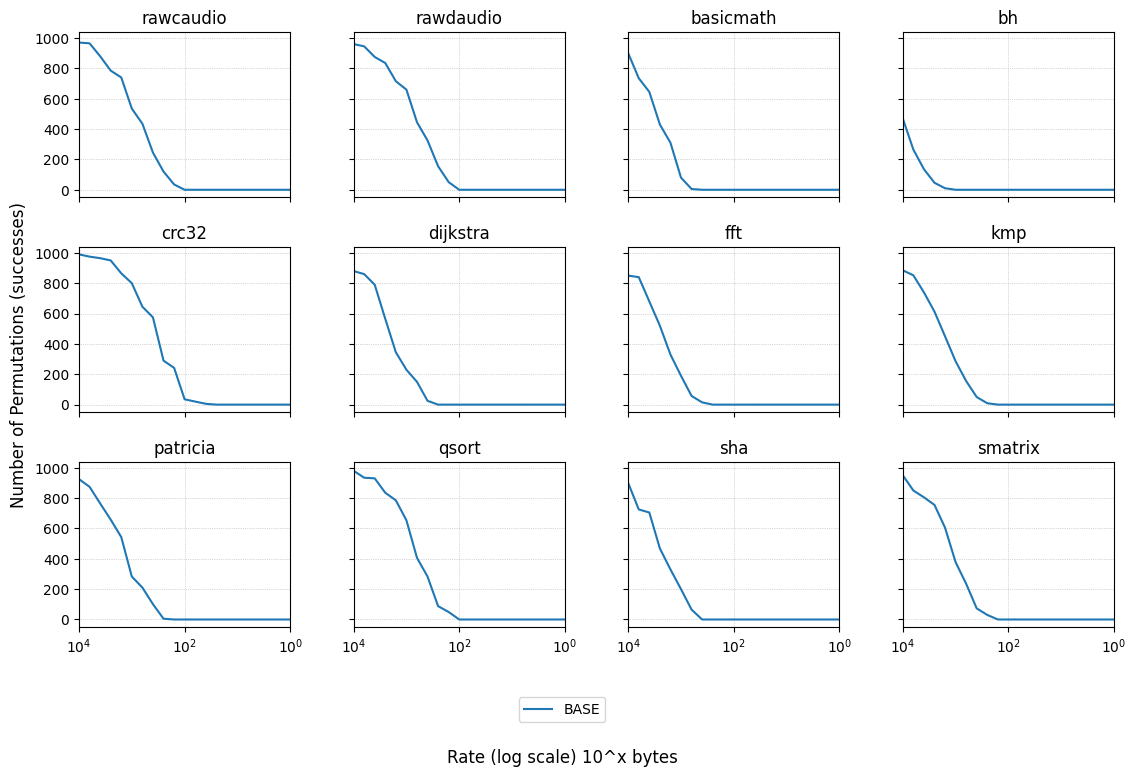
\includegraphics[width=0.90\linewidth]{Chapter-3/figs/baseline-reliability.png}
  \caption{Baseline limit study results showing reliability collapse as instruction faults increase. 
  Experiments executed on an Intel i7-8086K CPU (x86-64). 
  The x-axis shows the fault rate $\log_{10}(1/R)$; the y-axis shows the number of successful trials. 
  Reliability declines sharply once the expected number of corrupted instructions per program 
  approaches one.}
  \label{fig:baseline-reliability}
\end{figure}

\section{Interpretation}
\label{sec:limit-study-interpretation}

These results demonstrate that instruction memory is intrinsically fragile under persistent corruption.  
Even minimal, random instruction-level faults can permanently compromise system behavior, 
converting recoverable upsets into deterministic failures.  
Because the corrupted bytes persist across reboots, recovery through reset or replay is impossible; 
the system re-executes the same broken instruction sequence each time.

The baseline analysis therefore represents the natural limit of system reliability when no protection mechanisms are present.  
It defines a lower bound against which more advanced approaches can be compared.  
To surpass this boundary, a system must not only detect corruption but also regenerate usable code from damaged storage.  
Achieving this requires mechanisms capable of reconstructing functional instruction sequences directly within static memory---without reboot or external recovery.

\medskip
\noindent
The next chapter introduces one such approach: \textbf{recovery by repair}.  
Rather than leaving persistent faults unaddressed, repair techniques use redundancy and structured encoding 
to regenerate program content from corrupted data.  
This shift---from passive failure to active reconstruction---marks the first step toward self-sustaining reliability 
in persistent instruction memory.